%
%
%

\begin{figure}[t]
\begin{center}
\includegraphics[scale=0.5,angle=0]{figures/Noise_PerKid_MM18423_20121122_208_216.ps}
\caption{NEFD distribution for the two arrays (1.25 mm
  top, 2.14~mm bottom) during the  2012 observation campaign, for the MM18423 scans. The detector
  sensitivity is presented as a function of the KID number, sorted
  according to the resonance frequency. The average NEFD of the two arrays are
  48 and 23~mJy.s$^{1/2}$ at 1.25 and 2.14~mm, respectively, for these
  observations. If we consider only the best 20\% detectors of each array,
  then we get an average NEFD of 39 and 15~mJy.s$^{1/2}$.}
\label{fig:NEFDrun5}
\end{center}
\end{figure}

%noise map per kid satisfies Gaussian histogram (assumes regular spread of
%integration time and factor 2 for noise correlation between pixels with 4
%neared grid point method). Then propagate the noise up to the final map.
% the point source flux is deduced with a least-square-fit method so is
% linear. Hence noise can be propagated.

The flux of a point source is measured via a 2D Gaussian fit in the final average map with a fixed
width and a fixed position. The fit is linear and
involves a constant background, evaluated in a square area with a size of
ten times the FWHM of the Gaussian distribution, in our case 13~arcsec
(resp. 18~arcsec) at 1.25~mm (resp. 2.14~mm). A photometric correction (of
the order of 5~\%) is applied to the flux measurement to account for the
filtering effect induced by the TOI processing.

The noise equivalent flux density (NEFD) is computed as the array-averaged
sensitivity to point sources {\it i.e.} the flux rms obtained in one second of
integration. The average is done via the reciprocal of the square of the
NEFD. It takes the time effectively spent by the array on
the source into account.\\
Figure~\ref{fig:NEFDrun5} presents the NEFD for each valid KID of the array at
1.25~mm (top) and 2.14~mm (bottom) obtained during the observation of
MM18423+5938.  In this case, the average sensitivities on the sky are $\sim
48$ and $\sim 23$ mJy.s$^{1/2}$ at 1.25 and 2.14~mm, respectively. We note that
the sensitivity distribution variation across the array is quite large with the majority of detectors concentrated at the better sensitivity end. If we consider only the best 20~\% detectors of each array,
  then we get an average NEFD of 39 and 15~mJy.s$^{1/2}$.
  

Figure \ref{fig:NEFDfull} presents the array-averaged NEFD of the \NIKA\ camera
at 1.25 and 2.14~mm as a function of the line-of-sight opacity $\tau/
sin(\delta)$, where $\tau$ is the zenith opacity and $\delta$ the
elevation. The NEFD measurements are  obtained during the
observations described in Table~\ref{tab:table_sed}.  At zero zenith opacity,
the array-averaged NEFD are $\sim 40$ and $\sim 23$ mJy.s$^{1/2}$ at
1.25 and 2.14~mm, respectively, which give an indication of the performance of the 2012
\NIKA\ camera in optimal weather conditions.  As expected, the sensitivities
degrade with increasing opacity, corresponding to worse weather conditions. At
2.14~mm, we observe, as expected, a degradation due to the opacity effect, following 
$exp(\tau/sin(\delta))$, while the degradation seems to be
enhanced at 1.25~mm. Nevertheless, the sky noise decorrelation seems to work  in those
cases as well. We therefore confirm that the increased power on kids somehow reduces
their performance.

The sensitivity at 1.25~mm was limited by a saturation effect on the
readout electronics, which has been corrected since. By only using eight
detectors, we have been able to detect  the faint source MM18423. In that
case, the measured, averaged 1.25~mm NEFD is 27~mJy.s$^{1/2}$ to be compared with 48~mJy.s$^{1/2}$ for the full-array observation 
(fig.~\ref{fig:NEFDrun5}). 
%which is better
%to MAMBO-2 \citep{Lestrade:2009ef}, the predecessor of \NIKA\ at the 30\,m telescope. 
%We think that this sensitivity is representative of the 1.25\,mm array, although this is not
%demonstrated yet.


SXDF1100.001 has been observed twice during this observation campaign, with two different integration times 
(68 and 258 min), and we
used it to have a first estimate of the evolution of NEFD and noise with integration time. 
We note that the noise integrates down because the NEFD is stable, and the noise is divided by a 
factor 2 when increasing the integration time by a factor 4.


The 2013  observation campaign allowed us to test new arrays. Although an additional filter
has limited the 1.25~mm band efficiency, we were able to measure the 
array-averaged NEFD for two sources (HFLS3 and MM18423) in weather conditions far from 
optimal ($\tau$ up to 0.6).  As shown in figure \ref{fig:NEFDfull}, the achieved sensivities are much better (about 1/3 lower) 
and do follow an expected exponential trend. We extrapolate a sensitivity 
at zero zenith opacity of $\sim 40$ mJy.s$^{1/2}$ at 1.25~mm and $\sim 14$ at 2.14~mm. This improvement is related to technological parameters optimization 
as explained in section \ref{dac}.

 
In conclusion, the \NIKA\ instrument has shown an array-averaged NEFD on the sky for point sources of 
40 and 14~mJy.s$^{1/2}$ at 1.25 and 2.14~mm in optimal weather conditions. If we consider typical NIKA observing conditions (zenith opacity = 0.1, air mass = 1.5) the array-averaged NEFD results 46~mJy.s$^{1/2}$ at 1.25~mm channel and 15~mJy.s$^{1/2}$ at 2.14~mm channel. 
Hower, we expect the 1.25~mm channel sensitivity to be improved in the next  observation campaigns.

\begin{figure}[t]
\begin{center}
\includegraphics[scale=0.45]{figures/plotNEFD.eps}
\caption{Array-averaged NEFD as a function of the line-of-sight opacity $\tau/
sin(\delta)$. Black dots (resp. red squares) refer to the 1.25~mm array (resp. 2.14~mm) for the 2012 observation campaign, during which 
the trend at  2.14~mm is compatible with a $exp(\tau/sin(\delta))$ behavior (as shown with the red curve),
 while a departure from this behavior is observed at  1.25~mm. The latter can be attributed to the  degradation of the KID resonance quality
  factor with increasing power load. Open circles (resp. open squares) refer to the 1.25~mm array (resp. 2.14~mm) for the 2013 observation campaign. Very few points have been measured,  but the achieved sensivities are much better and do follow an expected exponential 
  trend.}
\label{fig:NEFDfull}
\end{center}
\end{figure}


\begin{table*}
\begin{center}
\begin{tabular}{lllrrrrr}
\hline
\hline
Source name & RA & Dec & $F_{\nu}\mathrm{(1.25~mm)}$ & $F_{\nu}\mathrm{(2.14~mm)}$       & $T_{int} (min)$ &  $\tau_{1}$ & $\tau_{2}$ \\
\hline
            & 2000 & 2000 &mJy          &mJy              & min      &              & \\
\hline
HLS091828     &  09:18:28.600  &  +51:42:23.300 & $36.7   \pm  4.6$  & $8.3 \pm 0.7 $   & 83 & 0.27 & 0.22 \\
%MM18423$^*$   &  18:42:22.500  &  +59:38:30.000 & $29   \pm  4$  & $5.5 \pm 0.7 $   & 56 & 0.02 & 0.01 \\
MM18423       &  18:42:22.500  &  +59:38:30.000 & $33.6   \pm  3$  & $6.3 \pm 0.8 $   & 37 & 0.02 & 0.03 \\
%MM18423$^{r6}$ &  18:42:22.500  &  +59:38:30.000 & $20  \pm  2$ & $4.3 \pm 0.3 $  & 26 & 0.56 & 0.34 \\
%SXDF          &  02:18:30.600  &  $-$05:31:30.000 & $20   \pm  3$  & $4.1 \pm 0.8 $   & 68 & 0.02 & 0.02 \\
SXDF          &  02:18:30.600  &  $-$05:31:30.000 & $28   \pm  1.5$  & $4.1 \pm 0.4 $   & 258& 0.03 & 0.03 \\
HFLS3$^{r6}$   &  17:06:47.800  &  +58:46:23.000 & $16   \pm  2$  & $4.0 \pm 0.6 $  & 16 & 0.14 & 0.07 \\ \hline
Arp220        &  15:34:57.100  &  +23:30:11.000 & $243  \pm  3 $  & $52.8  \pm 0.8 $   & 47 & 0.11 & 0.09 \\
HAT084933     &  08:49:33.400  &  +02:14:43.000 & $13   \pm  3$  & $1.3 \pm 0.8 $   & 59 & 0.08 & 0.07 \\
HAT133008     &  13:30:08.560  &  +24:58:58.300 & $16   \pm  3$  & $4.5 \pm 0.8 $   & 55 & 0.14 & 0.10 \\
PSS2322+1944  &  23:22:07.200  &  +19:44:23.000 & $<4.6         $  & $<1.7          $   & 57 & 0.06 & 0.05 \\
GRB121123A    &  20:29:16.290  &  $-$11:51:35.900 & $<15        $  & $<1.7          $   & 69 & 0.22 & 0.18 \\
4C05.19       &  04:14:37.800  &  +05:34:42.000 & $<6.2        $   & $26.3 \pm 0.8          $   & 15 & 0.13 & 0.11 \\
ZZTauIRS      &  04:30:51.714  &  +24:41:47.510 & $77  \pm  2$   & $16.2  \pm 0.8 $   & 40 & 0.01 & 0.00 \\
CXTau         &  04:14:47.865  &  +26:28:11.010 & $<4.6      $   & $<1.7          $   & 40 & 0.02 & 0.01 \\
\hline \hline

\end{tabular}
\end{center}
\caption{\NIKA\ Flux and sensitivity of a collection of point sources. 
The integration time is given in minutes. 
The average zenith opacities are given in the last two columns for the two
\NIKA\ wavelengths. 
Upper limits are given as $2~\sigma$. 
Most of the data were taken from 19 to 24 November 2012. 
%SXDF field was observed twice (22nd and 23rd of November 2012). 
%$^*$~Data taken with a different setting (8 Kids only at 1.25 mm). 
%$^{r6}$~Data taken in June 2013.
}
\label{tab:table_sed}
\end{table*}

% 4C: Remi's values
